% Graph for Workflow CARS
% usage: pdflatex workflow.tex && convert -density 200 workflow.pdf workflow.png && rm workflow.log workflow.aux workflow.pdf

\documentclass[preview]{standalone}
\usepackage{tikz}
\usetikzlibrary{shapes,arrows}
\pgfdeclarelayer{background}
\pgfdeclarelayer{foreground}
\pgfsetlayers{background,main,foreground}

% Define block styles
\tikzstyle{block} = [rectangle, draw, fill=blue!20, 
    text width=7em, text centered, rounded corners, minimum height=4em]
\tikzstyle{line} = [draw, -latex']
\tikzstyle{data} = [draw, ellipse,fill=red!20,
    text width=7em, text centered, minimum height=4em]
\def\checkmark{\tikz\fill[scale=0.4](0,.35) -- (.25,0) -- (1,.7) -- (.25,.15) -- cycle;} 

% Draw background
\newcommand{\background}[5]{%
  \begin{pgfonlayer}{background}
    % Left-top corner of the background rectangle
    \path (#1.west |- #2.north)+(-1em,3em) node (a1) {};
    % Right-bottom corner of the background rectangle
    \path (#3.east |- #4.south)+(+1em,-1em) node (a2) {};
    % Draw the background
    \path[fill=yellow!20,rounded corners, draw=black!50, dashed]
    (a1) rectangle (a2);
    
    \path (a1.east |- a1.south)+(6em,-1em) node (u1)
          {\textit{#5}};
\end{pgfonlayer}}
% --------------------------------------------------------------------------

\begin{document}

\begin{figure}
  \begin{minipage}[b]{.48\linewidth}
    \centering
    \resizebox {1\textwidth} {!}{
      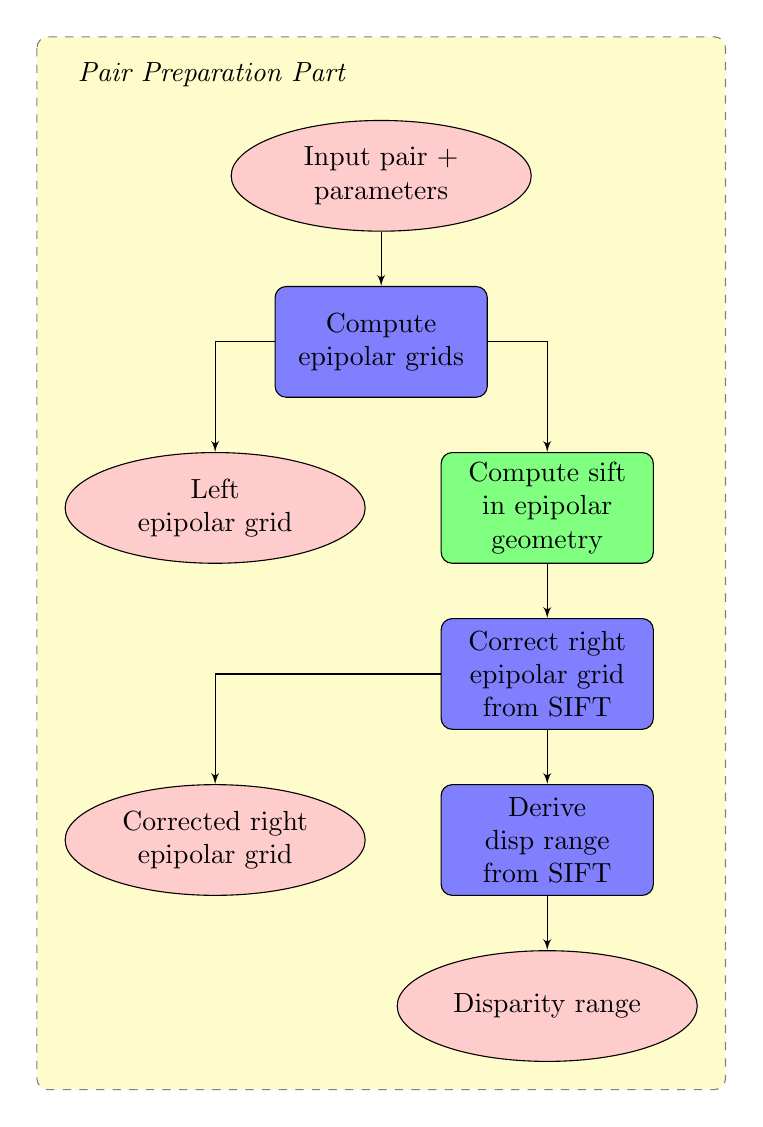
\begin{tikzpicture}[node distance = 6em, auto]
        % Place nodes
        
        % 1. Compute stereo-rectification grids for the input pair
        \node [block, fill=blue!50!white] (grid) {Compute epipolar grids};
        \node [data, above of=grid] (inpu) {Input pair + parameters};
        
        \node [below of=grid] (vir0){}; % virtual node for grid output
        \node [data, left of=vir0] (left) {Left \\ epipolar grid};
        
        % 2. Compute all possible sift matches in epipolar geometry
        \node [block, right of=vir0, fill=green!50!white] (sift) {Compute sift in epipolar geometry};
        
        % 3. Derive a bilinear correction model of the stereo-rectification grid for right image in order to minimize epipolar error
        % 4. Apply correction to right grid
        \node [block, below of=sift, fill=blue!50!white] (corr) {Correct right epipolar grid from SIFT};
        
        \node [below of=left] (vir1){}; % virtual node for sift output
        \node [data, below of=vir1] (righ) {Corrected right epipolar grid};

        % 5. Derive disp range from sift
        \node [block, below of=corr, fill=blue!50!white] (rang) {Derive disp range from SIFT};
        \node [data, below of=rang] (disp) {Disparity range};
        
        % Draw edges
        \path [line] (inpu) -- (grid);
        \path [line] (grid) -| (left);
        \path [line] (grid) -| (sift);
        \path [line] (sift) -- (corr);
        \path [line] (corr) -| (righ);
        \path [line] (corr) -- (rang);
        \path [line] (rang) -- (disp);
        \background{left}{inpu}{disp}{disp}{Pair Preparation Part}[]
        
      \end{tikzpicture}
    }
    \centerline{\scriptsize{(a) Prepare part}}\medskip
  \end{minipage}
  \hfill
  \begin{minipage}[b]{0.48\linewidth}
    \centering
    \resizebox {1\textwidth} {!}{
      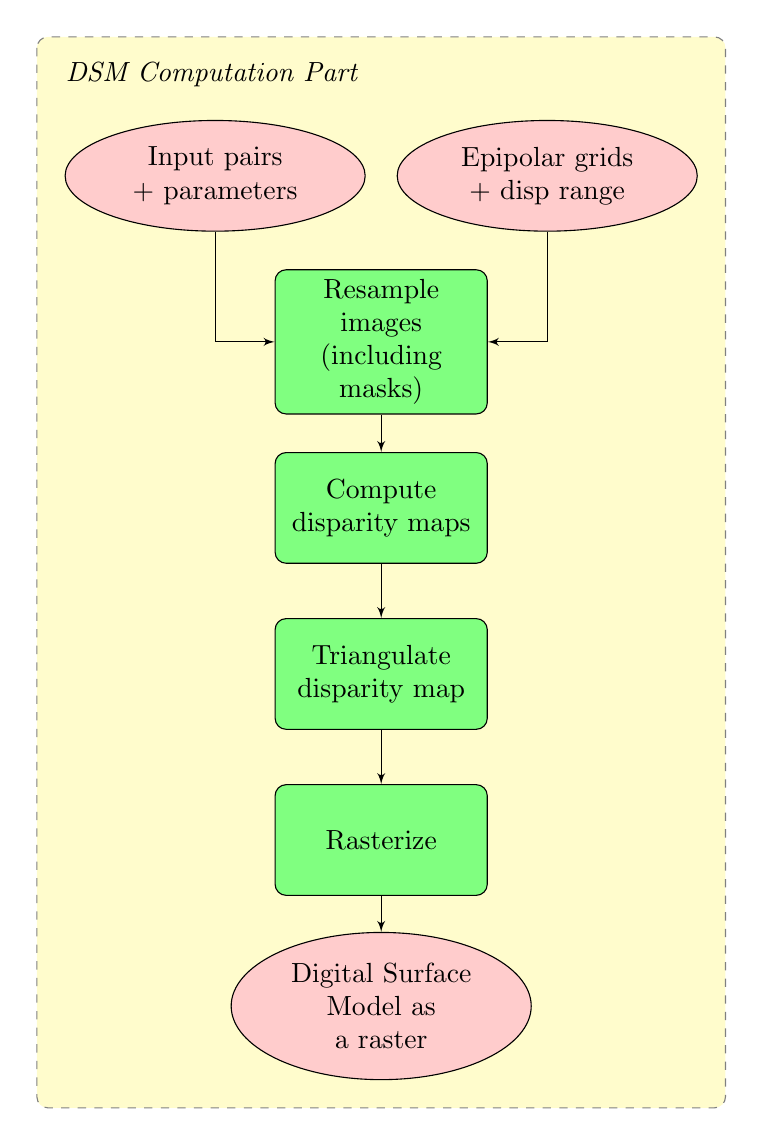
\begin{tikzpicture}[node distance = 6em, auto]
        % Place nodes
        % 1. Epipolar resampling (including mask)
        \node [block, fill=green!50!white] (resa) {Resample images \\(including masks)};
        
        \node [above of=resa] (vir0) {}; % virtual node for input
        \node [data, left of=vir0] (inpu) {Input pairs + parameters};
        \node [data, right of=vir0] (prep) {Epipolar grids + disp range};
        
        % 2. Disparity map estimation using Pandora (SGM)
        \node [block, below of=resa, fill=green!50!white] (disp){Compute disparity maps};
        
        % 3. Triangulation of disparity map
        \node [block, below of=disp, fill=green!50!white] (tria){Triangulate disparity map};
        
        % 4. Rasterization to DSM
        \node [block, below of=tria, fill=green!50!white] (rast){Rasterize};
        \node [data, below of=rast] (dsmo) {Digital Surface Model as a raster};
    
        % Draw edges
        \path [line] (inpu) |- (resa);
        \path [line] (prep) |- (resa);
        \path [line] (resa) -- (disp);
        \path [line] (disp) -- (tria);
        \path [line] (tria) -- (rast);
        \path [line] (rast) -- (dsmo);
        
        \background{inpu}{inpu}{prep}{dsmo}{DSM Computation Part}[]
        
      \end{tikzpicture}
    }
    \centerline{\scriptsize{(b) Compute DSM part}}\medskip
  \end{minipage}
\end{figure}

\end{document}
